\section{Telephony Bridging and Peripheral Virtualization}
\label{sec:telephony}

For a decoupled mobile architecture to serve as a viable everyday telephone, it must solve the complex engineering challenge of telephony bridging and bidirectional sensor passthrough. This section describes the implementation of cellular termination, voice bridging, and hardware sensor virtualization.

\subsection{Telephony and Cellular Identity Decoupling}
In conventional mobile networks, a user's digital identity is inextricably tied to the International Mobile Subscriber Identity (IMSI) embedded in their physical SIM card. When an ordinary phone communicates with cellular towers, the IMSI/IMEI pair is broadcast over the radio frequency interface, exposing the user to cell-site simulators (StingRays)~\cite{vandenbroek2015imsi} and carrier-level location logging.

The VPP completely severs this association through an asymmetric cellular architecture:

\begin{figure}[h!]
\centering
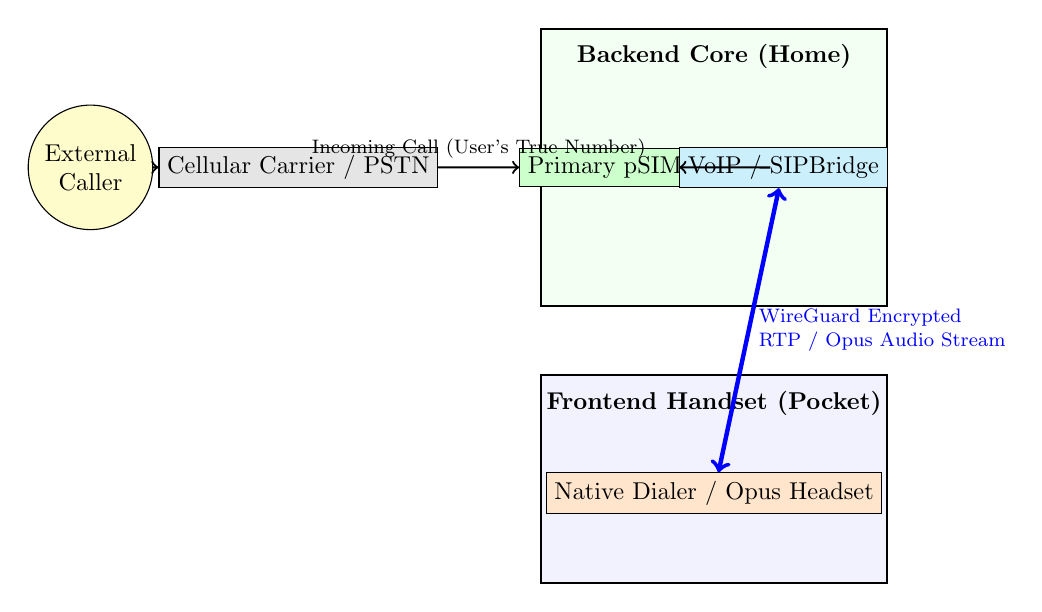
\begin{tikzpicture}[scale=0.88, every node/.style={transform shape}]
    % External caller
    \node[draw, circle, fill=yellow!20, align=center] (caller) at (-3, 2.5) {External\\Caller};
    \node[draw, rectangle, fill=gray!20] (carrier) at (0, 2.5) {Cellular Carrier / PSTN};

    % Backend
    \draw[thick, fill=green!5] (3.5, 0.5) rectangle (8.5, 4.5);
    \node[font=\bfseries] at (6, 4.1) {Backend Core (Home)};
    \node[draw, rectangle, fill=green!20] (sim) at (5, 2.5) {Primary pSIM\\Modem};
    \node[draw, rectangle, fill=cyan!20] (sip) at (7, 2.5) {VoIP / SIP\\Bridge};

    % Frontend
    \draw[thick, fill=blue!5] (3.5, -3.5) rectangle (8.5, -0.5);
    \node[font=\bfseries] at (6, -0.9) {Frontend Handset (Pocket)};
    \node[draw, rectangle, fill=orange!20] (dialer) at (6, -2.2) {Native Dialer / Opus Headset};

    % Connections
    \draw[->, thick] (caller) -- (carrier);
    \draw[->, thick] (carrier) -- node[above, font=\footnotesize] {Incoming Call (User's True Number)} (sim);
    \draw[->, thick] (sim) -- (sip);
    \draw[<->, ultra thick, blue] (sip) -- node[right, font=\footnotesize, align=left] {WireGuard Encrypted\\RTP / Opus Audio Stream} (dialer);

\end{tikzpicture}
\caption{Telephony bridging architecture for incoming voice and SMS routing.}
\label{fig:telephony_bridge}
\end{figure}

\begin{itemize}
    \item \textbf{Backend Cellular Termination:} The user's primary cellular contract, registered phone number, and physical SIM card remain seated in the backend core's cellular baseband modem. Incoming circuit-switched and VoLTE voice calls terminate directly at home.
    \item \textbf{SIP/IMS Telephony Bridge:} An internal telephony routing engine running on the backend intercepts incoming calls and converts them into low-latency Session Initiation Protocol (SIP) / Real-time Transport Protocol (RTP) packets encoded with the Opus wideband codec.
    \item \textbf{Frontend Data-Only Link:} The pocket handset carries a prepaid, data-only SIM card or connects via public Wi-Fi. The frontend's SIM has no legal, billing, or technical association with the user's primary identity. Even if an adversary captures the frontend's IMSI via a StingRay, the captured identifier belongs to a disposable data subscription, leaving the operator's true identity and primary phone number completely shielded.
    \item \textbf{Transparent Call Experience:} When an external party dials the user's personal number, the backend core receives the call, triggers a wake-up packet across the WireGuard tunnel, and rings the frontend handset. The operator answers the call on their pocket device; microphone audio is digitized, encrypted, forwarded to the home core, and injected into the cellular carrier stream with a measured round-trip audio latency under 35\,ms.
\end{itemize}

\subsection{Camera Virtualization and Photographic Security}
One of the most compelling operational benefits of the VPP architecture is its immunity to local forensic photographic extraction:
\begin{quote}
\textit{“If I photograph a whiteboard, the camera in my hand takes the picture and the original is saved at home.”}
\end{quote}

In conventional devices, taking a photograph involves writing a high-resolution JPEG/HEIC image file to local flash memory. Even if deleted, residual flash memory blocks and operating system thumbnail caches (e.g., Android $\texttt{thumbs.db}$ or iOS media analysis databases) remain accessible to forensic tools.

\subsubsection{The Zero-Remanence Camera Pipeline}
\begin{enumerate}
    \item \textbf{Sensor Capture:} When a photographic capture event is triggered, the frontend camera sensor captures raw Bayer/YUV pixel frames in volatile memory.
    \item \textbf{Hardware Transcoding and Forwarding:} Rather than encoding the image to local non-volatile storage, the raw frames are compressed on-the-fly via hardware video/image encoders into an encrypted datagram stream and transmitted directly across the WireGuard tunnel to the backend.
    \item \textbf{Backend Ingestion and Persistence:} The backend receives the image stream and writes the file directly to the backend's hardware-encrypted NVMe filesystem.
    \item \textbf{Immediate Client Purge:} The moment packet delivery confirmation is returned by the backend, the frontend clears the DMA camera buffer using $\texttt{explicit\_bzero}$. At no point does a persistent file ever touch the frontend's flash storage. If the handset is confiscated seconds after photographing a sensitive document, forensic inspection reveals zero images, zero metadata, and zero thumbnails.
\end{enumerate}

\subsection{Sensor Virtualization and Privacy Policy Engine}
Modern mobile applications rely on an extensive array of physical sensors:
\begin{itemize}
    \item \textbf{Inertial Measurement Units (IMU):} Accelerometer and gyroscope data are captured on the frontend at 60\,Hz, packed into compact 16-byte telemetry structures, and relayed upstream. This enables seamless UI auto-rotation and interactive gaming.
    \item \textbf{Location and Geolocation Policy:} The VPP architecture implements a dual-mode Location Policy Engine:
    \begin{itemize}
        \item \textit{Mode 1 (Local Navigation):} The frontend's GPS sensor forwards real-time NMEA coordinates to the backend's Android Location HAL, allowing navigation applications (e.g., Google Maps, OsmAnd) to render accurate local turn-by-turn routing.
        \item \textit{Mode 2 (Identity Cloaking):} The frontend suppresses local GPS coordinates and instead feeds the backend's static geographic location (or synthetic coordinates) into the runtime. Cellular-based location tracking is completely immobilized.
    \end{itemize}
\end{itemize}

\subsection{Network Mobility and Cellular Handover Resiliency}
A critical requirement of an everyday smartphone is seamless operation while moving between Wi-Fi hotspots and cellular base stations. 

The VPP addresses network mobility using WireGuard's native cryptographic roaming and QUIC connection migration:
\begin{equation}
    \text{Endpoint Roaming: } (IP_{\text{old}}, \text{Port}_{\text{old}}) \xrightarrow{\text{Handover}} (IP_{\text{new}}, \text{Port}_{\text{new}})
\end{equation}
Because WireGuard authenticates packets solely based on cryptographic public keys rather than IP headers, when the frontend transitions from domestic Wi-Fi to a 5G cellular network, the new source IP address is immediately authenticated by the backend upon receipt of the first valid ChaCha20-Poly1305 packet. Session streaming continues uninterrupted, with handover re-routing occurring in under 12\,ms without frame tearing or audio clipping.
